\begin{fullwidth}
\section{Identifying Employment Scams \& Tax Scams} % Top level section
Scams such as employment scams and tax scams are becoming increasingly common and more sophisticated then ever before. In fact, the FTC recorded over 105,000 "business and job opportunity" scams in 2023. This is more than a five-fold increase over the past five years \autocite{Heath:2024}.

\begin{figure*}[H] % Use the figure* environment for full width figures
    \centering
    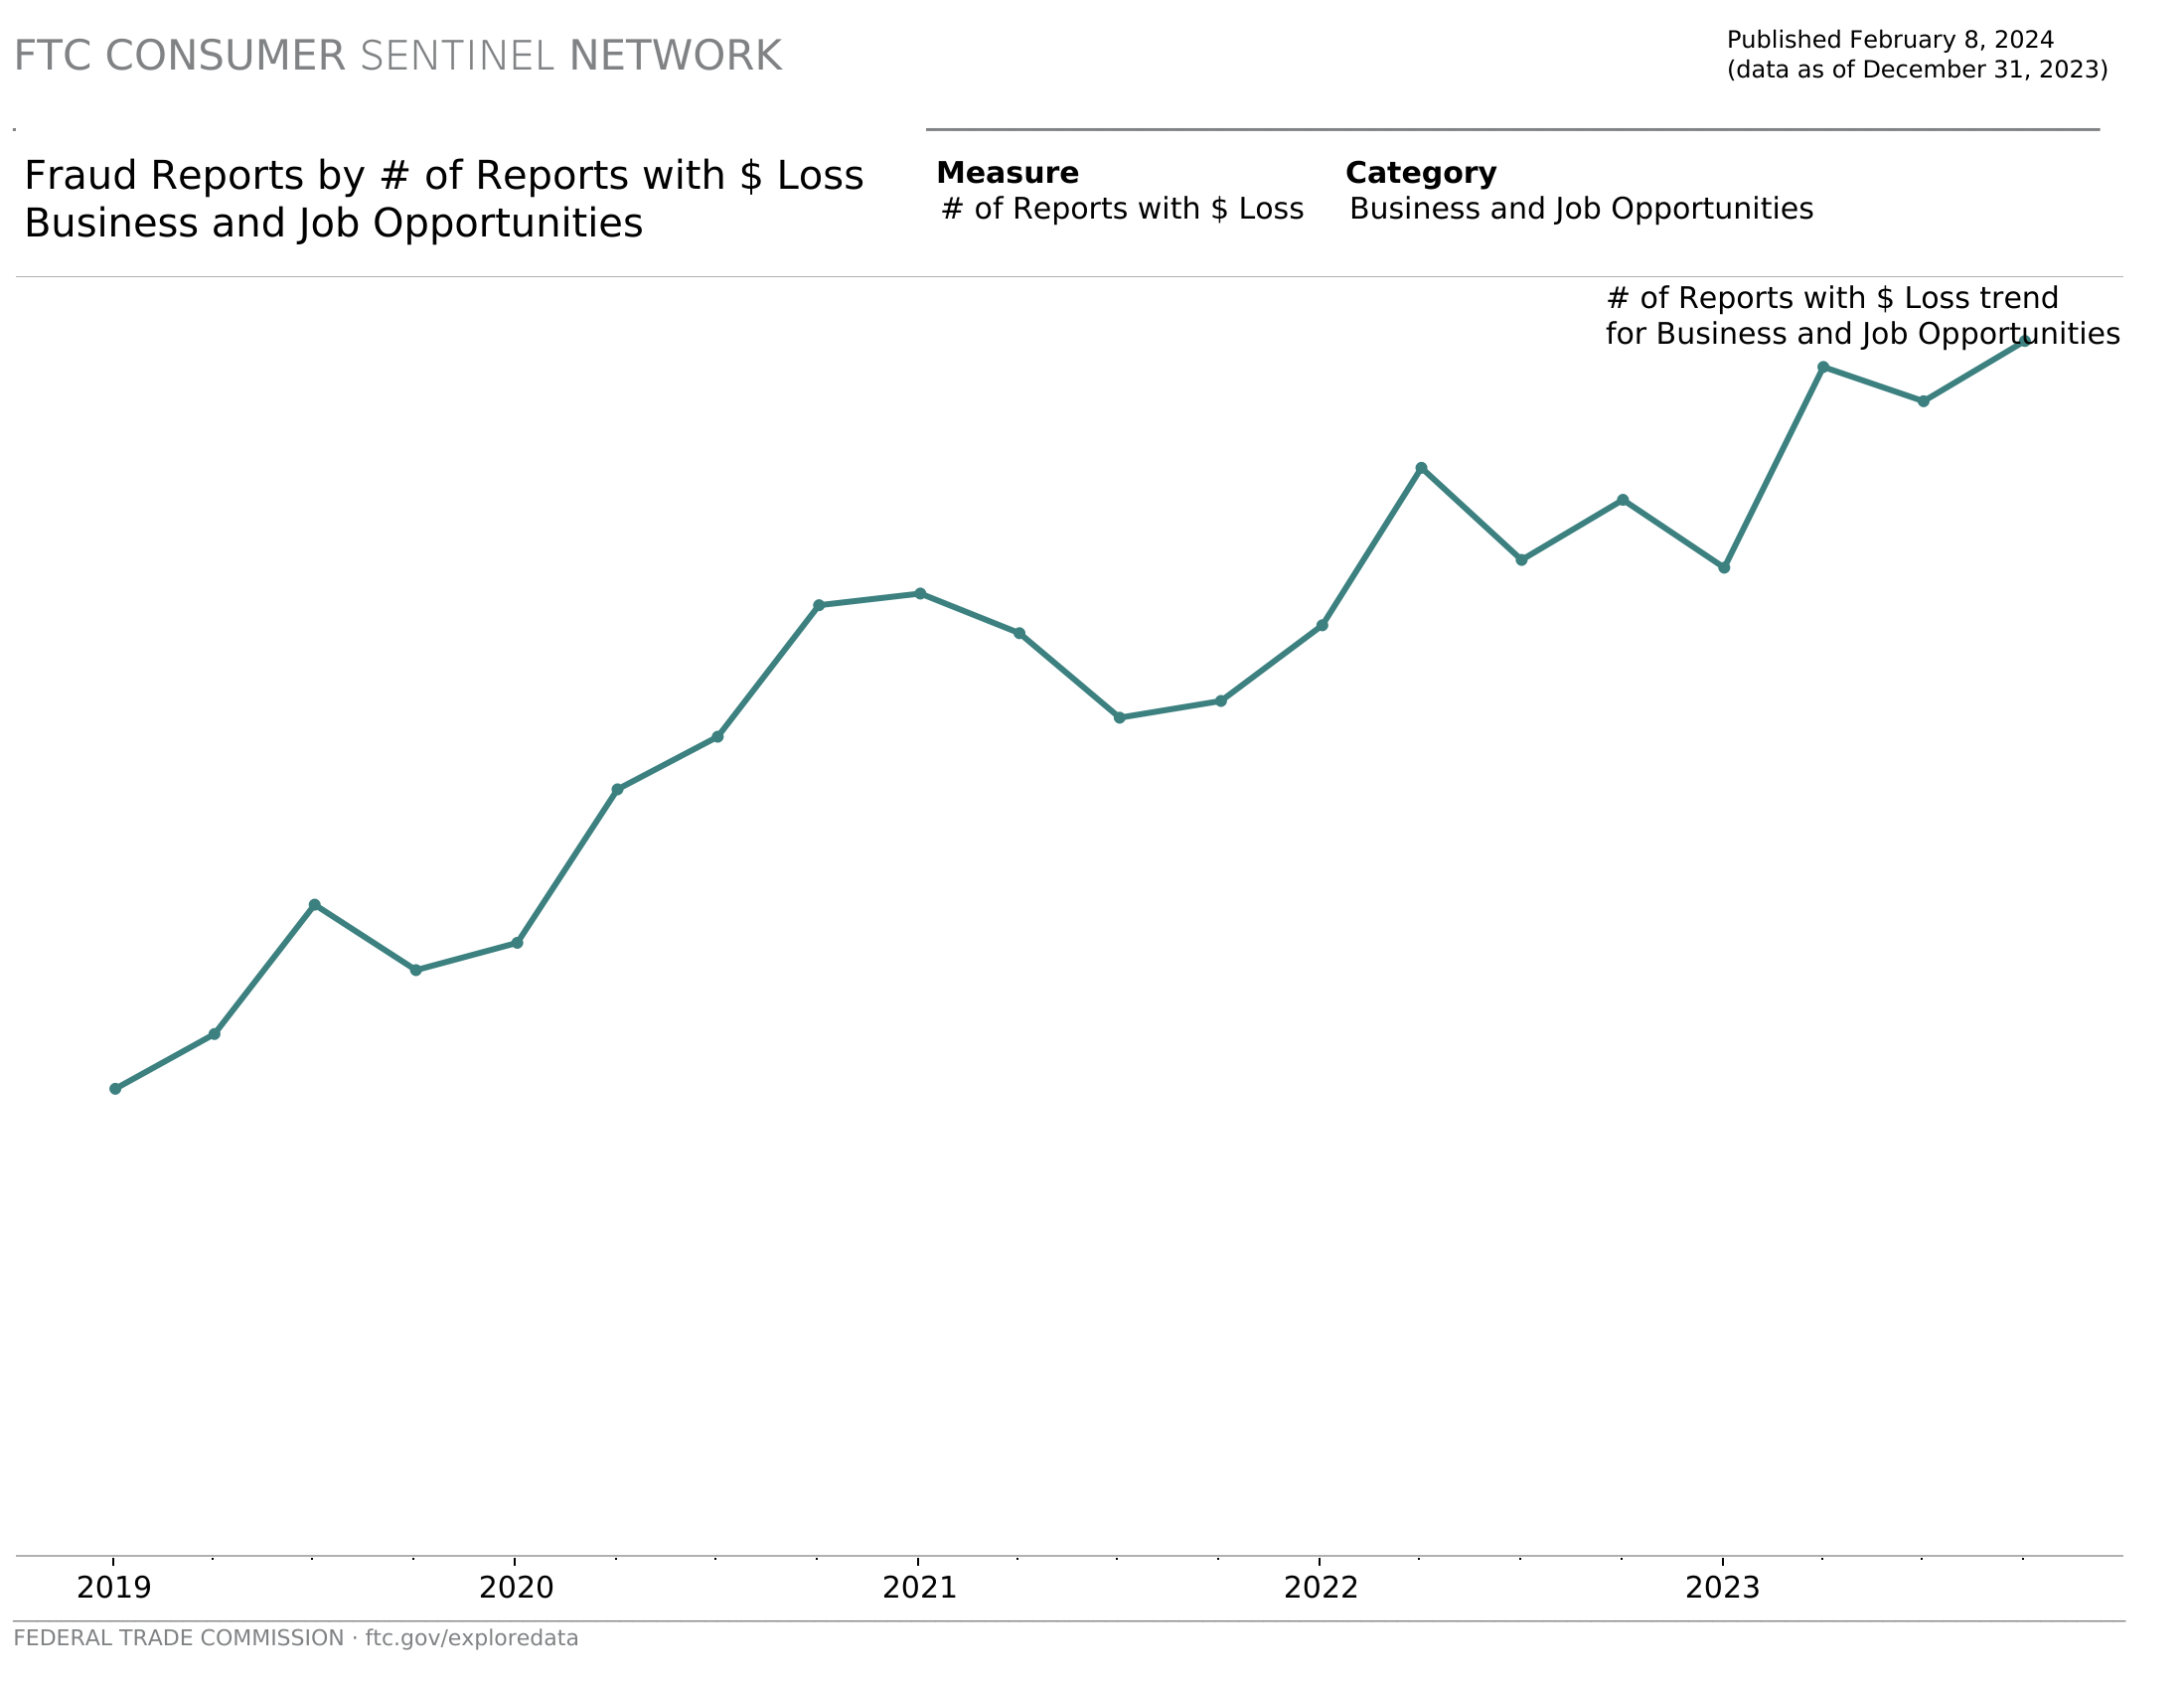
\includegraphics[width=.75\linewidth]{assets/Trends Over Time.png}
    \captionsetup{justification=centering}
    \caption{Number of fraud reports to the FCC with financial loss over time, \href{https://public.tableau.com/shared/HCT8WGQK8?:display_count=n&:origin=viz_share_link}{FCC Tableau}}
\end{figure*}

\subsection{General Scam Identification Steps} % Second level section

Scams usually attempt to exploit people for money or personal information such as a social security number. While there are various means and types of scams, the following are usually elements in a scam:

\begin{enumerate}
    \item \textbf{Pretending to be from a Common Organization}: A scammer may pretend to work for a large company or governmental entity that people know of to build trust.
    \item \textbf{Problem or Prize}: Scammers may pretend that the victim has a problem, such as jail time or debt. They also may tell the victim that there is a prize for completing the requested actions.
    \item \textbf{Pressure to Act}: Scammers want victims to act before they can think about the scam and identify it. They may threaten large fines or jail time.
    \item \textbf{Odd Payment Means}: Scammers may request payment through gift cards, cryptocurrency, or wire. These means are usually untraceable and you wont be able to be refunded or cancel the transaction.
\end{enumerate}

\subsection{Employment Scam Identification} % Second level section
Job scams can be hard to spot as the scammer usually identify people on legitimate job posting websites. They may also put targets through interview processes and have the target perform other tasks to build trust. Then, they will attempt to exploit the target for information or money.

The following are red flags of a job scam:
\begin{itemize}
    \item \textbf{Contacted from a Personal Email}: A job scam is likely when a recruiter contacts you from a personal email instead of one from a company. For example, if you received an email from a @gmail.com domain, it is likely that it is a job scam.
    \item \textbf{Requests Payments}: When a person posing as a job recruiter requests payment for work items or training, it is likely a job scam. Particularly if the employer promises to repay for the items.
    \item \textbf{Asking For Personal Information Upfront}: When an employer asks for personal information upfront, such as bank account information or social security numbers, a scam is likely.
\end{itemize}
If you are ever unsure that you are dealing with the recruiter or a scammer, find the companies contact information on the internet and call or email them to ensure that you are speaking to one of their recruiters \autocite{Lazarus:2023}. 

\subsection{Tax Season Scams Identification} % Second level section

During tax season, many scammers are working hard to steal money or personal information posing as the IRS. These scams can be conducted over various communication channels such as email, SMS, social media, or phone \autocite{FCC:2023}.

\begin{figure*}[H] % Use the figure* environment for full width figures
    \centering
    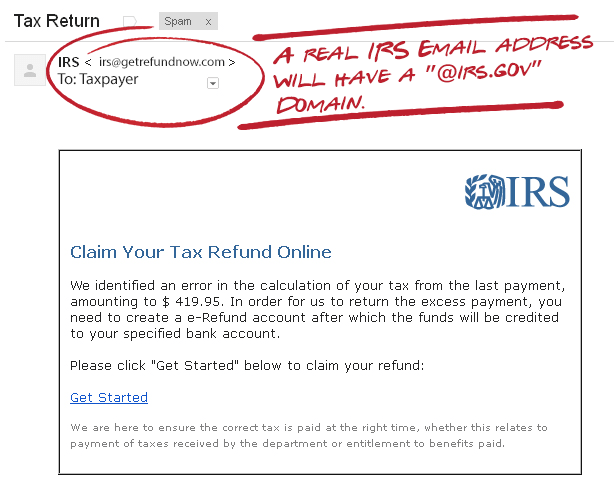
\includegraphics[width=.75\linewidth]{assets/example_tax_scam.png}
    \captionsetup{justification=centering}
    \caption{Common example of a tax scam, \href{https://www.michigan.gov/consumerprotection/protect-yourself/consumer-alerts/scams/irs-phone-email-tax}{Michigan Consumer Protection}.}
\end{figure*}

Signs of a tax season scam include:
\begin{itemize}
    \item \textbf{Phone Number Spoofing}: Scammers may use robocalls and phone number spoofing to make it appear that they are calling from a legitimate IRS phone number.
    \item \textbf{SMS Messages}: The IRS will not initiate contact with taxpayers via SMS. These messages often appear as urgent notifications with links.
    \item \textbf{Emails}: The IRS will not initiate contact with taxpayers via email. Any emails sent from the IRS will contain a .gov domain in the email address. Personal email addresses are never used for official contact.
\end{itemize}
To validate if the IRS is contacting you or if it is a scam, contact the IRS using the \href{https://www.irs.gov/help/let-us-help-you}{phone numbers listed on the official IRS website}. If the medium of contact is an email, you can forward it to \href{mailto:phishing@irs.gov}{phishing@irs.gov}.

\end{fullwidth}